\documentclass[letterpaper]{article}
\usepackage{graphicx}
\usepackage{siunitx}
\usepackage[hyphens]{url}
\usepackage{natbib}
\newcommand{\squared}{\textsuperscript{2}}
\date{2 October 2024}
\title{\emph{JED} Article}
\author{Joe Loughry}
\begin{document}
\maketitle
\begin{abstract}
It's not a covert channel because\ldots \\
It's not fault injection because\ldots \\
It's not a side channel because information runs in the other direction.
It's not the same as Light Commands because\ldots
\end{abstract}
\section{Impolite introduction}
Every covert channel paper ever starts off with the same implicit assumption:
\begin{quote}
{\it ``Grant us the inside man.''}
\end{quote}

\noindent We are asked to assume the system is already compromised. That we've
already bribed an operator, already tricked someone into plugging in a USB
containing our malware---assume we've already hacked into the system by
conventional means first---and then after that, you can do the bit with the
hovering drones.

But isn't that begging the question? It doesn't solve the first mile problem.
How do you get into an air-gapped system that wasn't already listening for a
signal? How do you get into a computer that hasn't been gimicked? Just an
ordinary computer, minding its own business.

\section{Key takeaway}

Assumptions matter.

We found this vulnerability because we went looking for it. Building on the
long history of side channels, it seemed reasonable that information could flow
the other way. This is a measurement paper. We hope others will find out how to
use it.

This article expands on our research paper presented at USENIX WOOT'24
\cite{Loughry2024b}, which is collaborative work with Kasper Rasmussen of the
University of Oxford.

What if you could do glitching attacks without access to the power supply? What
if you could do laser fault injection without boiling nitric acid and grinding
wheels, no longer limited to a microscope stage?

We show that
it is possible to do optical fault injection against a wide variety of electronic
devices in the wild. Anything with LED status indicators or relying on a shared
communication bus is potentially vulnerable.

The basilisk might be your spirit animal.

This is not a computer security vulnerability so much as it is a vulnerability
of the electronics underlying.

There are important limitations on this research. We have not demonstrated the
effect at long range. It works under laboratory conditions of access on
haywired devices; the only commercially available products found so far to be
vulnerable to the effect are garden decorations and a light-up dog toy.

This is a mesurement paper.

\section{History}:w

The specific vulnerability---optical fault injection exploitable from outside
the system at a distance---is as old as the IBM 701 (1952) and as current as
the Raspberry Pi 3 (2016).




This is a measurement paper.

Unlike most covert channel attacks on airgapped
systems, the first phase (1) network infiltration, of the Advanced Persistent
Threat (APT) kill chain, need not require the introduction of malware. No
insider threat is necessary.


We found this vulnerability because we went looking for it.

TODO: focus on things we can't do yet.

TODO: laser safety.

immediately after the bit
about supplying all the energy needed to run the electronics, note that these
are absolutely not eye safe lasers. We take elaborate precautions around them
including interlocks, protective goggles, warning signs, and radiation
shielding.

TODO: always answer the ``so what?'' question.

TODO: with reference to glitching, talk about the dog toy.

If the eyes are the windows to the soul, LEDs are a window into the electronics.

\section{Context}

So the context here is status indicator lamps.

If you shine a \emph{really} bright light on them, all that energy has to go
somewhere. Would you believe it flows backwards into the electronics? Effects
range from nothing at all, to remote code execution. It takes a fairly powerful
laser to do it, because in addition to information, you are supplying all the
energy needed to run the electronics in reverse.

By the way---that last point is important. The energy levels involved here are
high. These are absolutely not eye safe lasers. We take elaborate precautions
around them including interlocks, protective goggles, warning signs, and
radiation shielding. Be careful.

There are at least two different physical effects at work: a photoelectric
effect and a photoconductive effect. The photoelectric effect lets us change a
binary 0 to 1, but not the other way around. The photoconductive effect lets us
change a binary 1 to 0, but not the other way around. This immediately suggests
that the two effects might be used in concert, but the problem is some
electronic components respond only to one effect or the other, but not both.

\section{Instruction set and reachability graph}

This places some fascinating constraints on the attacker. Those bit
patterns in the table on the left are all the possible assembly language
instructions. If we assume you can only change a binary 0 to 1, but you can
never go the other way around, then some of those instructions are reachable
from other instructions, as you can tell from the graph on the right.

The attacker might be able to change a load instruction into a branch, or an
add into a subtract, but he can't change a branch into a store, or a divide
into a compare, so we say he can execute arbitrary-ish code. It's a kind of
weird machine. It's easy to redirect a memory access up into high memory---just
set the high bit of the address---so our attacker patiently watches the
instruction stream go by, picking and choosing opcodes he can alter into the
instructions he wants, slowly building up the desired program in high memory.
Maybe it's not quite the program he wanted, because certain bit patterns were
unreachable, so the first thing the arbitrary-ish code does is run fixups on
itself. Finally, we redirect a branch, and it's game over.

The attacker must be very careful not to crash the running program, because its
memory accesses are needed to subvert. If the target computer ever crashes,
access is lost.
\section{History}
It might be a good idea to put in the sum of the history here, distinguish from
covert channels, and cite \cite{Kuhnapfel2021b}.

This work is different from Light Commands because there, the computer was
listening for a signal \cite{Sugawara2019,Rampazzi2020}.
\section{Analysis}
Analysis begins with the electrical schematic of a device, looking for
potentially susceptible components in electrically interesting places. This is
one of the constraints on the attacker; we can't choose where are the LEDs are
or how they're connected, and that determines what we can do. Not every
indicator will do something useful if reversed.
\section{LEDs}
Here's an electronic component. Light emitting diodes are interesting because
they're a naked P--N junction, the basic building block of solid state
electronics. You put electricity in, light comes out---pink light, in this
case. But there's a general principle in physics that any process that runs in
one direction can usually be made to run in the other direction if you supply
enough energy to make up for the difference in entropy.

When you put light into an LED, it comes out as electricity but in the opposite
direction from the usual current that makes it light up. This violates
important assumptions made by the circuit designer. We can force the voltage on
a communication bus low---or high, depending on how the LED is connected---by
hitting it from a distance with a laser.

If the eyes are the windows to the soul, then LED status indicators are a
window into the electronics.
\section{This is a measurement paper}
The first question everybody always asks is, how far away can you do this. And
the answer is we don't know. I didn't put this in the paper, because of
anonymous peer review, but the reason we don't know is because I suck at
aiming. So we solved that problem. We aimed it once, and then bolted everything
down so it can't drift out of alignment. It's not my problem to figure out how
to aim this thing. It's my problem to measure it.

So we built this infernal machine. It consists of a pair of linear actuators,
the X axis one bolted crosswise atop the carriage of the Y axis one, which lets
us raster scan a focused laser across any desired component on the circuit
board, stopping every fiftieth of a millimeter to measure the voltage on the
communication bus. There's a live I2C bus under there, and it's communicating
the whole time. Each linear actuator has a stepper motor, and there's a bank of
relays that lets us automatically vary the bus voltage and pull-up resistor
value. The orange stuff is radiation shielding. Data collection is automatic,
transmitted out by a serial connection. The whole thing is controlled by an
Arduino.
\section{Data}
Here's what the raw data from one of those scans looks like. You're looking
straight on at the LED; the big blue square is exactly five millimeters across.
The curvy arc on the right hand side is an artifact of the dome lens on the
LED, we think.

We can draw isovoltage contours to begin to visualize how the voltage on the
communication bus varies as the laser scans across the face of the LED. We're
looking for the physical location where our laser can force the voltage on the
circuit to go below the logic threshold.

The only one we're interested in is the 2.0 volt contour line, because that's
the value we found by experimentation to be the critical value.

This picture is where Professor Rasmussen got all excited. He calls it the
active area. Any hit by the laser inside that region alters the value of a bit.
Anything outside that region is a miss.

He wanted to know the area inside that curve. This directly corresponds to how
hard the target is to hit.

You can kind of see the outline of the square chip in the LED, or maybe that's
just my imagination.
\section{But there's a problem}
There's a problem, though, with commercially available devices. Blinky lights
are cool, but the hardware designer might not have put one where we need it, on
the communication bus.

You can't shoot lasers at an LED that isn't there.
\section{Other photosensitive components}
But I don't want to give you the impression that it's only status indicators;
the definition of ``accessible P--N junction'' is wider than that. Here's a
microphotograph of the silicon chip inside an electrostatic discharge
protection (ESD) component like the one at the lower left---which are found on
shared communication buses, because they're susceptible to static
electricity---and are even more sensitive than LEDs. Yes, you need line of
sight.

Here you can see the results of a lot of repeated runs against one of those.
Notice how the active area, in red, gets larger as you move down the chart, and
as you move toward the right. As the system voltage decreases, from TTL to CMOS
to low-voltage CMOS, by the time we get down to 1.8 volt LVCMOS, on the bottom
row, we can force the value of a bit against any reasonable value of pull-up
resistor.

Note that the active area on this component is quite a bit smaller than an LED.
That's a microphotograph in the upper left corner. The chip is only about 125
microns across, and it's off-center in the gap. So it's a challenging target to
hit.

Now we have a model that makes testable predictions. For any combination of LED
color, laser wavelength, logic family, and pull-up resistor value, we can
predict if it's reversible.

It's not isotropic either; this plot shows the effect of elliptical beam axis
rotation on the active area. We have not looked into the effect of polarization
at all.
\section{Stealth}
By the way, LEDs respond to short wavelength visible lasers, but we found the
most effective laser wavelengths for silicon are in the invisible infrared,
outside visual range. This means the attack is stealthy.
\section{Commercially available devices}
Hit it with a fast pulse of infrared at \SI{900}{\nano\metre} and we can
reliably reset the sequence to red.

The headlines write themselves.
\section{Demonstration I}
This is a fairly simple computer; it implements the instruction set from the
previous slide, but it's complex enough to illustrate the difficulty. Four-bit
CPU, load/store architecture with one register called the accumulator, which is
visible on the front panel, which is important. That's the accumulator over on
the right hand side. Think of this as a factory automation controller, reading
temperatures and pressures, turning motors on and off to open and close valves
in a chemical process plant, say. Normal operation is shown by a regular
scanning pattern on the accumulator lamps, 1-2-3-4, 1-2-3-4. The attacker needs
to watch the target system for a while, to learn the timing and establish a
phase lock on the internal state of the CPU. This is possible because the
accumulator display always changes at a particular microcode cycle, which might
be different for different instructions that can change the value in the
accumulator, but the attacker can tell the difference between those
instructions by observing the direction and magnitude of the change. So the
attacker just watches, measuring the cycle time and getting a phase lock on the
microcode cycle. It takes about ten iterations through the program to get a
phase lock.

Timing is absolutely critical. Once the attacker has got a phase lock, the
lasers begin firing. The beam is invisible, because these are ultraviolet
lasers, but you might be able to see a little fluorescence in the clear epoxy
over the green LEDs in the middle. This also serves to illustrate the general
principle that you're not always watching the same LED you're shooting at. It
only takes a few seconds. But note that the pattern on the accumulator lamps
has changed. It's not doing the same regular 1-2-3-4-1-2-3-4 scanning pattern
as before. That's because the computer is now running a completely different
program, one that we put there through the status indicator lamps.
\section{Demonstration II}
Late breaking news. Here's proof of concept, running on a live I2C bus. The
owner of the system is trying to write the message NORMAL OPERATION on the
display; the laser is trying to write the message PROOF OF CONCEPT.

They're fighting for control of the bus, and the laser is generally winning.
\section{Technical notes}
Good engineering practice does not load down a high speed communication bus
with unnecessary parasitic components.

We found this because we went looking for it.

With reference to the Black Hat USA talk mentioned earlier, the dog toy
represents a new kind of glitching attack, done through indicators rather than
the power supply \cite{Beaumont2024a}.

Ours is more general than the usual glitching attack, which can only change the
return address; we can introduce our arbitrary code.

Glitching is usually introduced through the back door. We can extend to going
in through the front door.
\section{Detection of attack in progress}
\begin{figure}[ht]
  \centering
  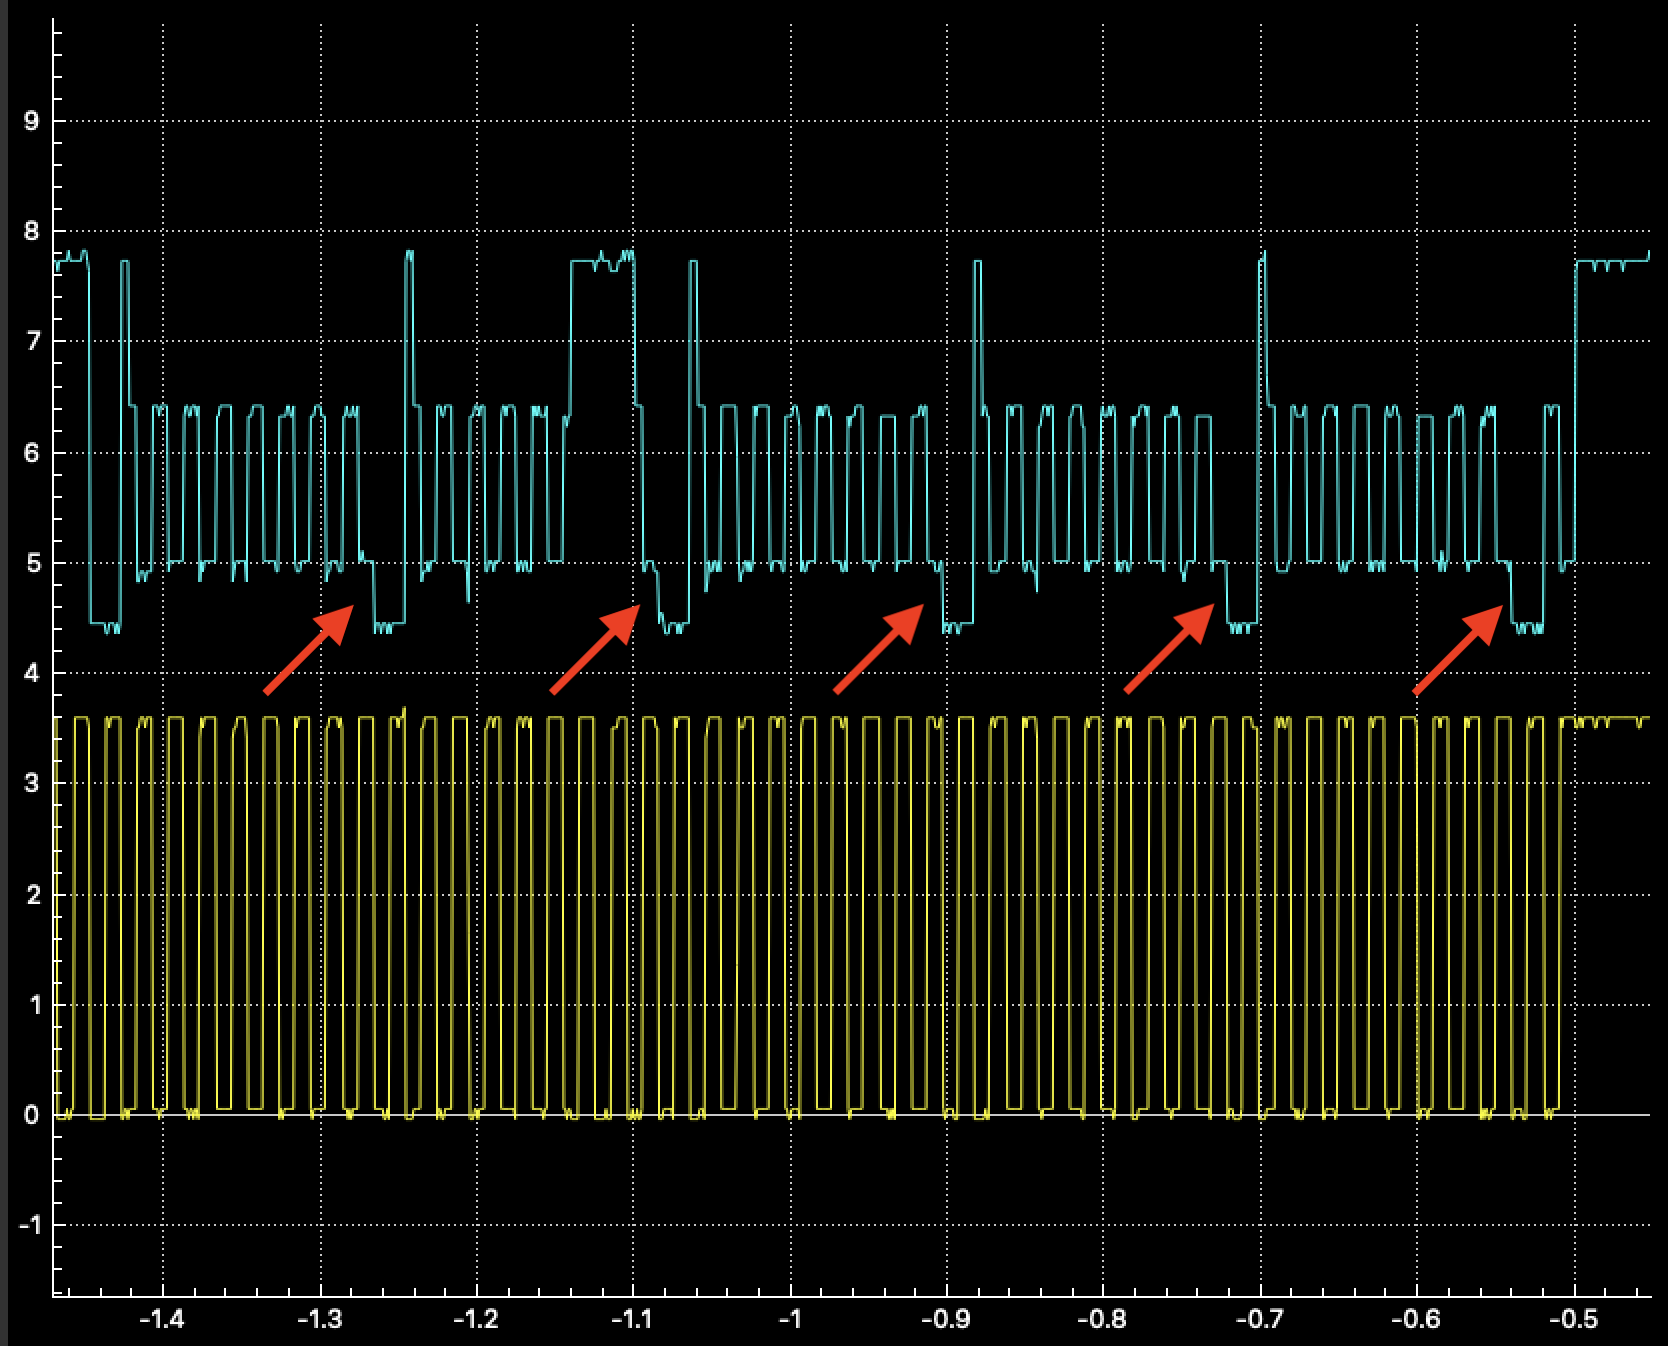
\includegraphics[width=\linewidth]{graphics/signature_of_the_attack.png}
  \caption{Negative-going acknowledgement pulses (red arrows) in the SDA signal
    are a distinctive signature of a successful photoconductive mode laser
    attack on an I\squared C bus.}
  \label{figure:attack_signature}
\end{figure}
Negative-going acknowledgement pulses, extending all the way ground
(Figure~\ref{figure:attack_signature}) are a distinctive signature indicating a
successful laser attack in progress on an I\squared C bus that is visible on an
oscilloscope \cite{Loughry2024c}. Their presence means that at least one
receiver on the I\squared C bus recognizes the laser as a legitimate sender and
has accepted a command from it.

\section{Arduino}
The Arduino Uno is bulletproof.

\cite{Guri2024c}.

\section{Summary and Conclusion}
Finally, I want to thank the anonymous peer reviewers for being so hard on us.
There is not one claim left in this paper that we did not measure to three
decimal places. It's a better paper because of it.

What did we overlook? Show us what angles we missed.
\bibliographystyle{unsrtnat}
\bibliography{consolidated_bibtex_file}
\end{document}
